%% Document class definition
\documentclass[aps, prd, reprint]{revtex4-2}
%
%% Include packages
\usepackage{graphicx}
\usepackage{amsmath}

% % % % % % % % % % % % % % % % % % % % % % % % %
% Corresponding author's email after affiliations
\usepackage{etoolbox}
\makeatletter
\def\@email#1#2{
 \endgroup
 \patchcmd{\titleblock@produce}
  {\frontmatter@RRAPformat}
  {\frontmatter@RRAPformat{\produce@RRAP{*#1\href{mailto:#2}{#2}}}\frontmatter@RRAPformat}
  {}{}
}
\makeatother
% % % % % %

%%%%%%%%%%%%
% Document %
%%%%%%%%%%%%
\begin{document}

% Title
\title{Supplementary Material (SM) for\\``Towards electrical domain-wall control in polyacetylene-based electronic nanodevices''}

%Authors and Affiliations
\author{Leandro M. Arancibia$^{\dagger\ddagger}$}
\author{Andrés I. Bertoni$^{\dagger\ddagger}$}
\author{Cristián G. Sánchez$^{\dagger}$}
\author{Alejandro M. Lobos$^{\dagger\,*}$}
\email[~Corresponding author.~E-mail:~]{alejandro.martin.lobos@gmail.com}
\affiliation{$^\dagger$~Instituto Interdisciplinario de Ciencias Básicas (ICB-CONICET), Universidad Nacional de Cuyo, Padre Jorge Contreras 1300, Mendoza 5502, Argentina}
\affiliation{$^\ddagger$~\normalfont These authors contributed equally to this work and are listed in alphabetical order.}

% Prints Title
\maketitle

% Body of the Supplementary Material
\section*{Section A}

In this section we will show that the contribution of the capacitive coupling term to the total energy is simply the electrostatic potential energy of the charges accumulated per gate due to the applied external voltage.

Our goal is to rewrite the total energy of the chain in terms of excess charges and external voltages. To this end, we start by writing the complete system Hamiltonian of Eq.~\ref{}, making explicit only the electronic term that introduces the effect of the external gate voltages:
\[
\hat{H} = \hat{H}^{0} + \sum_{n}^{N_{s}}\sum_{s} \mu_{n} \, c_{n,s}^{\dagger} \, c_{n,s}
\]
For ease of interpretation, we begin by defining the operator~$\hat{p}_{n}$, which corresponds to the observable electronic population per site~($p_{n}$):
\[
\hat{p}_{n} = \sum_{s} c_{n,s}^{\dagger} \, c_{n,s} \quad , \quad p_{n} = \left\langle \, \hat{p}_{n} \, \right\rangle
\]\[
\hat{H} = \hat{H}^{0} + \sum_{n}^{N_{s}} \mu_{n} \, \hat{p}_{n}
\]
From this, the associated total energy expression can be expressed as follows:
\[
E_{\mathrm{GS}} = \langle\, \hat{H} \,\rangle_{\mathrm{GS}} = \langle \, \Psi_{GS} \, | \, \hat{H} \, | \, \Psi_{GS} \, \rangle
\]\[
E_{\mathrm{GS}} = \langle\, \hat{H}^{0} \,\rangle_{\mathrm{GS}} + \sum_{n}^{N_{s}} \mu_{n} \, p_{n}
\]
The above energy expression allows us to more easily make explicit the excess charge per site, $q_{n}$, which can be interpreted as the net charge per site (${q_{n} = q^{\text{ion}}_{n} - p_{n}}$) or as the charge resulting from the fluctuation of the electron density at each site with respect to the neutral reference in the absence of external voltages (${q_{n} = -(p_{n} - p_{n}^{0})}$), since both interpretations give identical expressions (as ${q^{\text{ion}}_{n} = p_{n}^{0} = 1}$):
\[
q_{n} = 1 - p_{n}
\]
Note that the sign convention of this definition of charge allows a direct physical interpretation: excess electron density results in a net negative charge, and electron depletion results in a net positive charge.

We then continue working on our expression for the total energy by replacing with (i) our definition of excess charge per site and (ii) with the values of $\mu_{n}$ according to our model of two anti-symmetric voltage gates (see Fig.~1 in the main manuscript):
\[
E_{\mathrm{GS}} = \langle\, \hat{H}^{0} \,\rangle_{\mathrm{GS}} + \sum_{n}^{N_{s}} \mu_{n} \, (1 - q_{n})
\]\[
E_{\mathrm{GS}} = \langle\, \hat{H}^{0} \,\rangle_{\mathrm{GS}} + \sum_{n \in g^{+}}^{w_{g}} (+V_{g}) \, (1 - q_{n}) + \sum_{n \in g^{-}}^{w_{g}} (-V_{g}) \, (1 - q_{n})
\]
Which simplifies to:
\[
E_{\mathrm{GS}} = \langle\, \hat{H}^{0} \,\rangle_{\mathrm{GS}} - \sum_{n \in g^{+}}^{w_{g}} V_{g} \, q_{n} - \sum_{n \in g^{-}}^{w_{g}} (-V_{g}) \, q_{n}
\]
Finally, after recognizing the charge accumulated at the gate (${Q_{g} \ge 0}$), we can conclude that the capacitive coupling term contributes to the total energy with the electrostatic potential energy of these excess charges per gate due to the applied external voltage:
\[
Q_{g} = \pm \sum_{n \in g^{\pm}}^{w_{g}} q_{n}
\]\[
E_{\mathrm{GS}} = \langle\, \hat{H}^{0} \,\rangle_{\mathrm{GS}} - 2\, V_{g} \, Q_{g}
\]
The factor $2$ appears because our model works with two anti-symmetric voltage gates (i.e., of equal width, opposite applied voltage, and equal distance from the center of the chain).

\newpage

\onecolumngrid
\section*{Section B}
%
\begin{figure}[h!]
    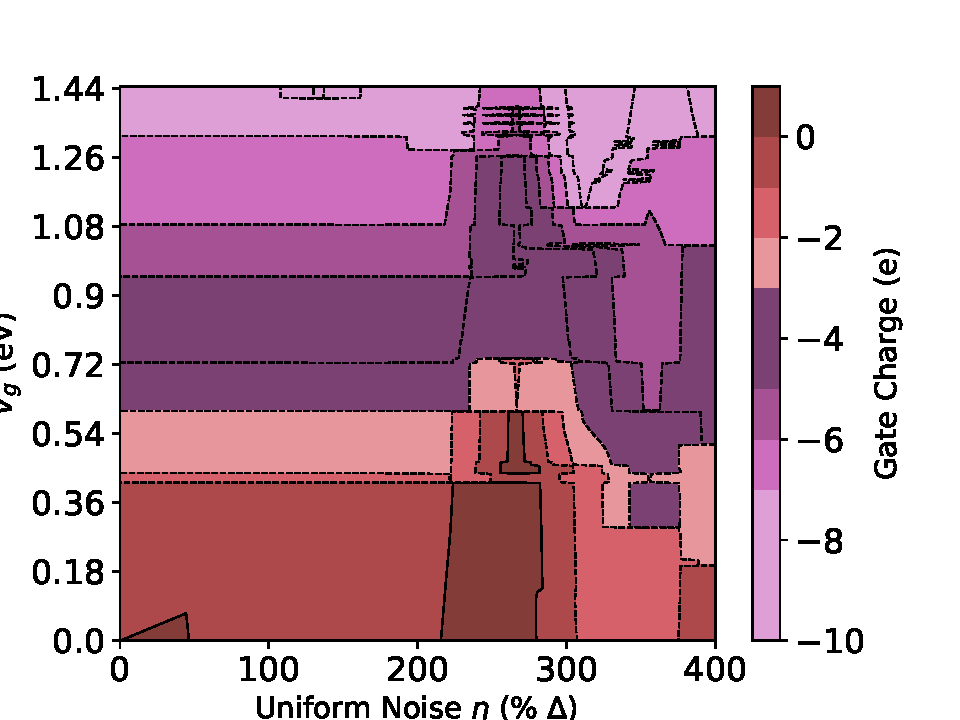
\includegraphics[scale=0.7]{figures/noise_contourmap.pdf}
    \label{fig:noise}
\end{figure}
%
Phase diagram of the stable solutions, labeled by their number of DWs, for different levels of uniform random noise (in units of percentage of the Peierls gap, $Delta$) applied to the externally applied voltage $V_{g}$; we used the same color coding as in the color bar of Fig. ~2 in the main manuscript. The added noise models the unintended fluctuations of the applied voltage profile $\mu_{n}$, which may result from normal room temperature fluctuations or aspects related to the non-ideality of an experimental setup. Notice that the system is remarkably robust to strong noise in $V_{g}$ (up to two times $Delta$); this result promotes the realistic feasibility of fabricating this device for use in technological applications.
\end{document}
